\section{Experimental results}
Many real world datasets contain missing values, often encoded as blanks, NaNs or other placeholders. Missing data imputation (MDI) has therefore long been a popular problem to tackle in statistics and machine learning~\cite{little1986statistical, nelwamondo2007missing}, and recently GNNs have proved to be a powerful tool~\cite{spinelli2020neural} for the task. With a view that our method incorporates additional higher-dimensional structure in the data, we evaluate the performance of the SNNs in imputing missing data over simplicial complexes.

%\subsection{Dataset description}
\textbf{Dataset description.} The datasets we analyze are extracted from the Semantic Scholar Open Research Corpus~\cite{ammar18NAACL}. The data contains over $39$ million published research papers together with their authors and numbers of citations. We retained only papers with more than $5$ citations and at most $10$ authors. As is common in TDA, we preprocess our data by constructing a simplicial complex. Our work focuses on \emph{co-authorship complexes} (or \emph{collaboration complexes})~\cite{patania2017}, simplicial complexes where a paper with $k$ authors is represented by a $(k-1)$-simplex \gard{We need to say something about how we interpret the subsimplices of a paper here.}. We constructed different co-authorship complexes by considering subsamples of the Semantic Scholar dataset. The subsamples were obtained by performing random walks (of length $80$) on the nodes of the graph which vertices corresponds to papers and edges connect papers sharing at least one author. We believe this extracts representative data from the dataset. The co-authorship complexes obtained from each subsampling have corresponding $k$-cochains given by the number of shared citations of the given collaboration (see Figure~\ref{fig:data2complex}).

\textbf{Method.} We evaluate the performance of the SNNs on the task of imputing missing data on the $k$-cochains (for $k=0,1,2$) of the extracted co-authorship complexes. As in a typical pipeline for this task~\cite{nelwamondo2007missing}, missing data is artificially introduced by replacing a portion of the values with a constant. Specifically, given a fixed co-authorship complex missing, data is introduced at random on the $k$-cochains at $4$ rates: $10\%,  20\%,  30\%$, and $50\%$. The training input is then given by the $k$-cochains where the random missing data is substituted by the median of the known data (the median is perhaps a reasonable first guess for estimating missing data). We trained an SNN comprising $3$ layers with $30$ convolutional filters of degree $5$. We used the $L_1$ norm as reconstruction loss over the known elements, and the Adam optimizer with a learning rate of $10^{-3}$. The SNN was trained for $1000$ iterations \gard{Should we specify the batch size?}. We then test the performance of the network on its accuracy in imputing missing data. As a statistical evaluation, we tested the network on different random samples of the damaged portions for the same percentage of missing values (see Section~\ref{sec:supp_material} (B)). 

%\subsection{Results}
\textbf{Results.} \gard{Note for me to remember to add a punchline somewhere in this section :-)} The results in Figure~\ref{fig:accuracy-error} (a-b) show the MA and MAE of the SNN in inputing missing citations on CC1 (Co-authorship Complex 1, for statistics on the complex see Table~\ref{table:Simplices-coauthor}, Section~\ref{sec:supp_material}). Observe that the distribution of the prediction error accumulates close to zeros.
%\begin{figure}[htbp]
%  \centering
%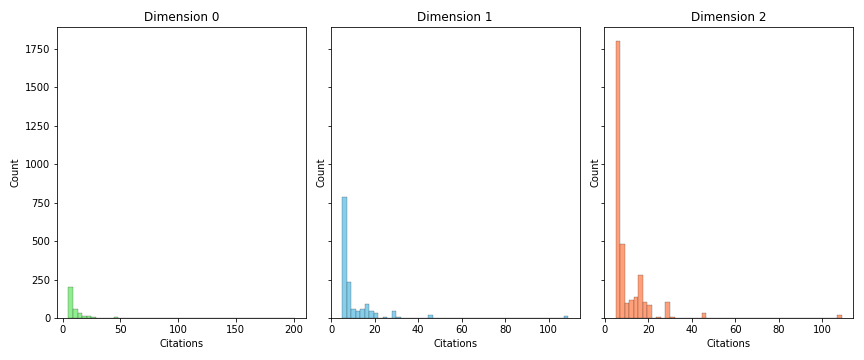
\includegraphics[scale=0.35]{./figures/distribution_cohain_150250.png}
% \caption{Distribution of the citation in CC1 } \label{fig:accuracy}
%\end{figure}
\begin{figure}[tb]
\centering
 \begin{subfigure}[t]{-0.8\textwidth}
 \vspace{-4cm}
    \text{(a)}
  \end{subfigure}
\begin{subfigure}[t]{0.8\textwidth}
\centering
   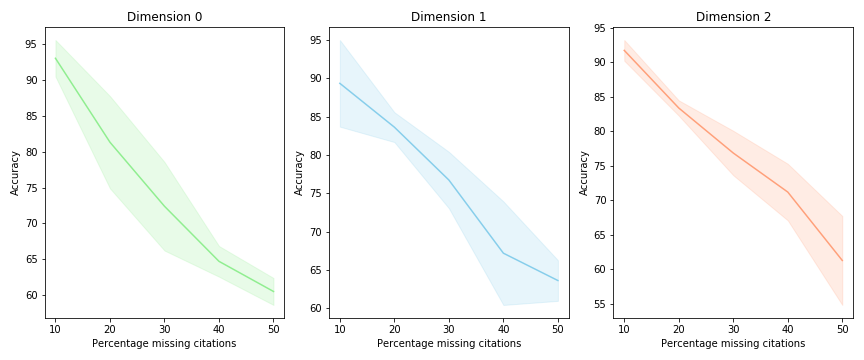
\includegraphics[scale=0.35]{./figures/accuracy_network1.png}
 %\caption{Accuracy of SNN in predicting missing citations } \label{fig:accuracy}
\end{subfigure}
 \begin{subfigure}[t]{0.8\textwidth}
    \text{(b)}
  \end{subfigure}
\begin{subfigure}[t]{0.8\textwidth}
\centering
\vspace{-0.5cm}
   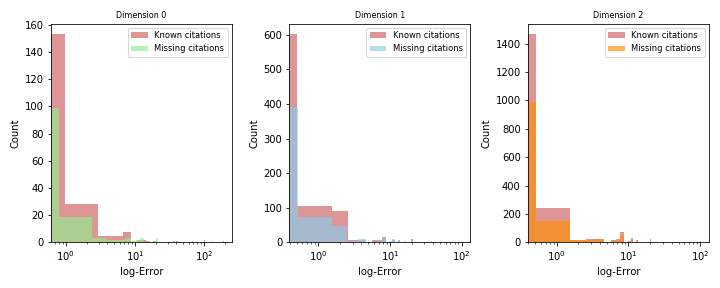
\includegraphics[scale=0.36]{./figures/Error_dist_start150250_seed6666_notsee40.png}
 % \caption{Distribution of the prediction's error} \label{fig:error}
\end{subfigure}
\caption{(a) Mean Accuracy $\pm$ std over 5 samples of SNN in imputing missing citations on CC1. (b)Mean Absolute Error $\pm$ std over 5 samples of SNN for $40\%$ missing values in CC1. \stefania{Add error on bins}}
\label{fig:accuracy-error}
\end{figure}
As a second assessment for our network we evaluate how accurately an SNN pretrained on a co-authorship complex can impute missing citations on a different complex. This is build over the assumption that co-authorship complexes share a similar structure. In Figure~\ref{fig:transfer-learning} we show the MA in predicting missing citations on CC1 using the above architecture of SNN trained on CC2 (Co-authorship Complex 2, see Table~\ref{table:Simplices-coauthor}, Section~\ref{sec:supp_material}).
We compared our results with imputation methods based on statistical techniques, namely replacing missing data with the median or mean of the known data and inferring the missing values from the $(k-1)$ and $(k+1)$ neighbors of the simplices ($k$-simplicial neighbor $k$-sn). As Table~\ref{table:comparison-SNN} shows, SNNs outperform statistical techniques. Comparison with other state of the art imputations algorithms is left for future work.
\begin{figure}[htbp]
  \centering
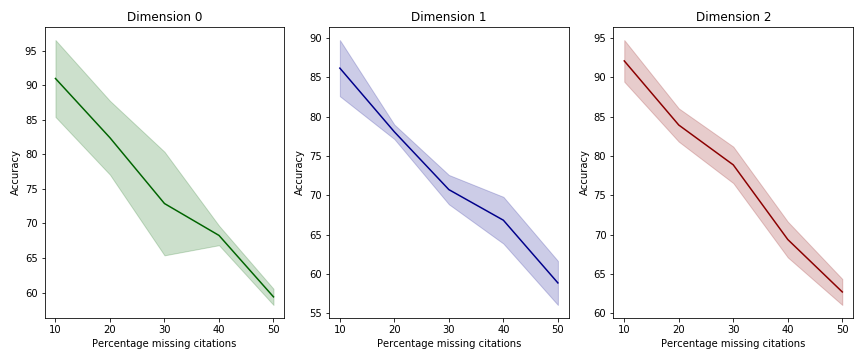
\includegraphics[scale=0.35]{./figures/accuracy_network1_pretrained.png}
  \caption{ Mean Accuracy $\pm$ std over 5 samples in imputing missing citations on CC1 of SNN trained on CC2 . } \label{fig:transfer-learning}
\end{figure}

%\scriptsize{
\begin{table}[htbp]
  \centering
  \scriptsize{
  \begin{tabular}{c|cccccc}
    \cmidrule(r){1-7}
    Method   & CC1 - dim 0   & CC1 - dim 1   & CC1 - dim 2   & CC2 - dim 0  & CC2 - dim 1  & CC2 - dim 2 \\
    \midrule
    Mean & $3.3 \pm 0.82$ & $5.75\pm 1.28$  &$ 2.96\pm 0.49$  & $3.32 \pm 0.85$ & $8.31 \pm 1.03$  & $7.90\pm 0.35$\\
    Median & $7.78 \pm 0.7$   & $10.44 \pm 1.$ &$ 12.75 \pm 0.63 $ & $5.76 \pm 0.38 $&$ 6.3\pm 0.36  $&$ 6.11\pm 0.2$\\
    $k$-sn & $30.89\pm 5.47 $& $33.97 \pm 1.92$ & $39.43 \pm 0.83  $& $21.67 \pm 2.67 $&$ 29.26\pm 1.35$   &$ 32.36 \pm 0.5 $\\
    \bottomrule
  \end{tabular}}
   \vspace{2pt}
  \caption{%
 Mean Accuracy $\pm$ standard deviation for $30\%$ of missing data over 5 samples. \stefania{Add uniform distribution sampling instead of mean?}
  }\label{table:comparison-SNN}
\end{table}%}
